\section{Benchmarks Settings}
\label{sec:benchmark:framework-cmp}

This section describes the benchmark experiments which aim to compare the
techniques introduced by AFOR with the compression methods described in
Section~\ref{sec:compression:state-of-the-art}. The first experiment measures
the indexing performance based on two aspects:
\begin{inparaenum}[(1)]
\item the indexing time; and 
\item the index size. 
\end{inparaenum}
The indexing time corresponds to the time required to build the index, be it a
traditional inverted index or a node-based inverted index like SIREn. As for
the index size, this time will vary with the compression technique used. The
second experiment compares the query execution performance using indexes built
with different compression techniques.

\paragraph{Data Collection}

In these benchmarks, five datasets were used. Two of them are plain text
datasets which will be used to build traditional inverted indexes, while the
three others are RDF triples and so will be used to build SIREn indexes.

\begin{quotation}
$\Longrightarrow$ Datasets for traditional indexes are composed of:
\begin{description}
\item[Wikipedia:] set of English language Wikipedia articles (~2.5 million
articles). Its total size is 42GB uncompressed.
\item[Blog:] set of 44 million blog posts made between August 1st and October
1st, 2008~\cite{burton:2009:spinn3r}. Its total size is 142GB uncompressed.
\end{description}
\end{quotation}

\begin{quotation}
$\Longrightarrow$ Datasets for the SIREn structure are the following three:
\begin{description}
\item[Geonames:] a geographical database and contains 13.8 million of
entities\footnote{Geonames: \url{http://www.geonames.org/}}. The size is 1.8GB
compressed.
\item[DBPedia:] a semi-structured version of Wikipedia and contains 17.7
million of entities\footnote{DBpedia: \url{http://dbpedia.org/}}. The size is
1.5GB compressed.
\item[Sindice:] a sample of the data collection currently indexed by Sindice.
There is a total of 130.540.675 entities. The size is 6.9GB compressed.
\end{description}
We extracted the entity descriptions from each dataset as pictured in
Figure~\ref{fig:entities}.
\end{quotation}

\section{Indexing Performance}
\label{sec:compression:indexing-performance}

The performance of indexing is compared based on the index size (compression
ratio), commit time (compression speed) and optimise time (compression and
decompression speed). The indexing is performed by adding incrementally 10000
documents at a time and finally by optimising the index.

We report the results of the indexing experiments in
Table~\ref{tab:indexing-performance}. The table comprises two columns with
respect to the indexing time: the total commit time (\emph{Total}) to add all
the documents and the optimisation time (\emph{Opt}). The time collected is
the CPU time used by the current thread and comprises the user time and the
system time. The index size in Table \ref{tab:indexing-performance} is studied
based on the size of each values' streams in the inverted file, and on the total
size of the index. For indexes built with unstructured data (i.e. Wikipedia and
Blog), these streams represent the document identifier, the frequency and the
positions. As for the indexes built on structured data (i.e. DBpedia, Geonames,
Sindice), the streams represent the entity, frequency, attribute, value and
position values. In each tables, the total size is computed by summing the size
of each streams. Bar plots are also provided in order to visualise better the
differences between the techniques.

\paragraph{Commit Time}

Figure~\ref{fig:commit-time} shows the total time spent by each method. As
might be expected, Rice is the slowest method due to its execution flow
complexity on both source type.

On the large unstructured dataset Blog, PFOR is equivalent to Rice in term of
compression speed, since PFOR spends more time in finding the outliers. AFOR-2
and S-64 perform similarly, while AFOR-1 performs as fast as VByte. The drop of
efficiency between AFOR-2 and AFOR-1 is due to the optimization algorithm to
find the best compressing frame. On the small dataset Wikipedia, Rice is
followed by S-64. While FOR, PFOR and VByte perform similarly, AFOR-1 and
AFOR-2 algorithms are the most efficient methods.

On small structured datasets (DBpedia and Geonames), algorithms behave
similarly as described previously. AFOR-3 shows equivalent performance as S-64
on DBpedia, while performing as the best one on Geonames. On a large dataset
(Sindice), VByte is the best-performing method while AFOR-1, AFOR-2, AFOR-3
and S-64 provide a similar commit time. On large datasets (Sindice and Blog),
VByte provides the best commit times, reflecting the benefit from a simple
algorithm.

\begin{figure}
  \centering
    \resizebox{0.8\linewidth}{!}{%
    % \subfloat[Unstructured data]{%
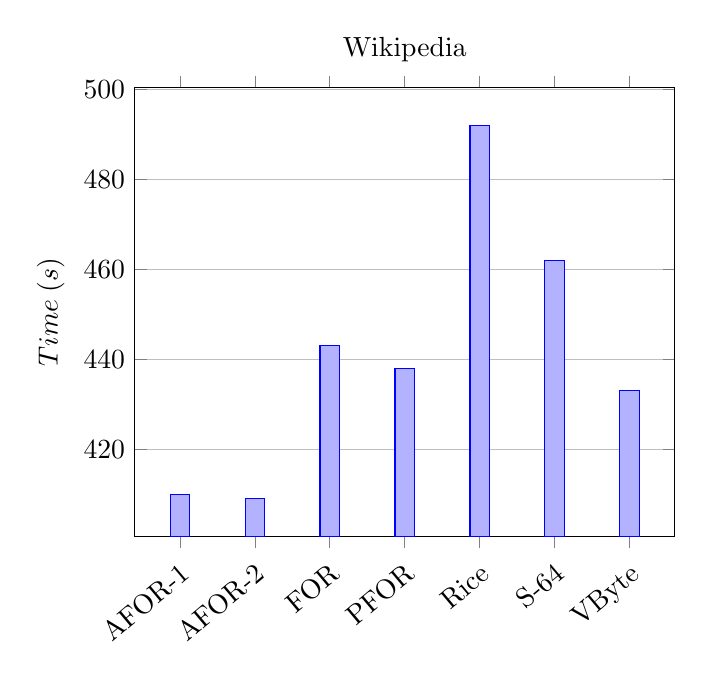
\begin{tikzpicture}[baseline]
\begin{axis}[
ylabel=$Time \; (s)$,
x tick label style={rotate=40, anchor=north east},
xtick={1,...,7},
xticklabels={AFOR-1, AFOR-2, FOR, PFOR, Rice, S-64, VByte},
legend style={at={(0.5,1.13)}, anchor=north, legend columns=-1},
ybar,
ymajorgrids=true,
bar width=7pt,
%enlargelimits=0.015,
title={Wikipedia}
]

\addplot
coordinates {(1, 410) (2, 409) (3, 443) (4, 438) (5, 492) (6, 462) (7, 433)};

\end{axis}
\end{tikzpicture}

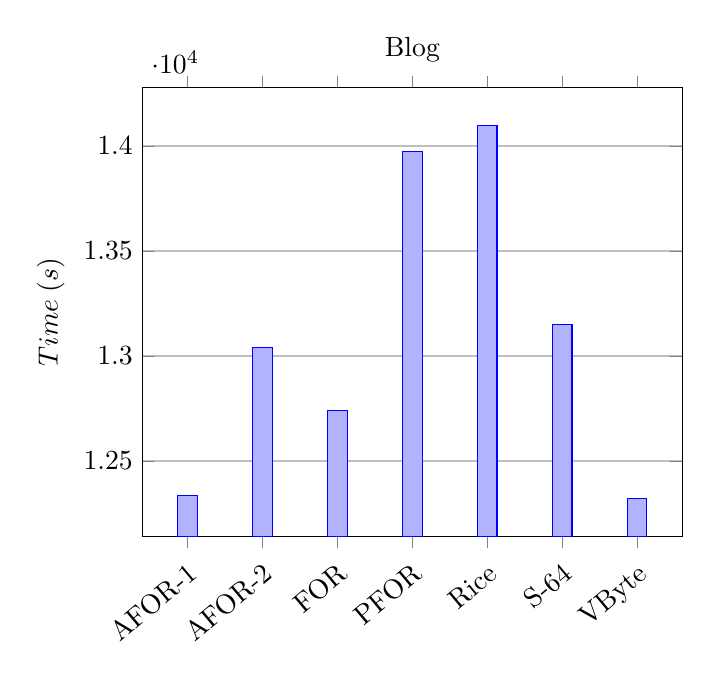
\begin{tikzpicture}[baseline]
\begin{axis}[
ylabel=$Time \; (s)$,
x tick label style={rotate=40, anchor=north east},
xtick={1,...,7},
xticklabels={AFOR-1, AFOR-2, FOR, PFOR, Rice, S-64, VByte},
legend style={at={(0.5,1.13)}, anchor=north, legend columns=-1},
ybar,
ymajorgrids=true,
bar width=7pt,
%enlargelimits=0.015,
title={Blog}
]

\addplot
coordinates {(1, 12337) (2, 13040) (3, 12741) (4, 13972) (5, 14099) (6, 13152) (7, 12320)};

\end{axis}
\end{tikzpicture}
% }
  }
\quad
  \resizebox{\linewidth}{!}{%
    % \subfloat[Structured data]{%
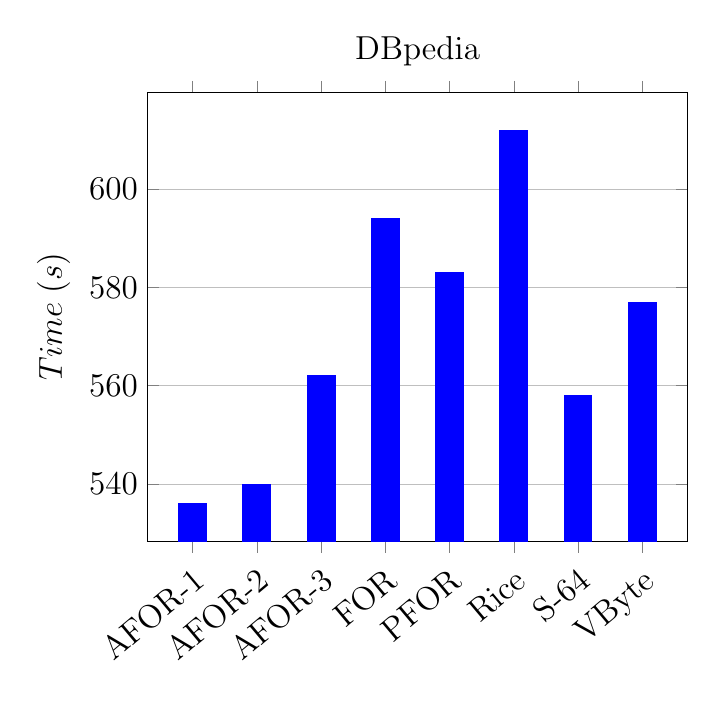
\begin{tikzpicture}[baseline]
\begin{axis}[
ylabel=$Time \; (s)$,
x tick label style={font=\large, rotate=40, anchor=north east},
xtick={1,...,8},
xticklabels={AFOR-1, AFOR-2, AFOR-3, FOR, PFOR, Rice, S-64, VByte},
legend style={at={(0.5,1.13)}, anchor=north, legend columns=-1},
label style={font=\large},
tick label style={font=\large},
title style={font=\large},
ybar,
ymajorgrids=true,
bar width=10pt,
title={DBpedia},
%enlargelimits=0.15,
]
\addplot[draw=blue,fill=blue]
coordinates {(1, 536) (2, 540) (3, 562) (4, 594) (5, 583) (6, 612) (7, 558) (8, 577)};
%\legend{Wikipedia}
\end{axis}
\end{tikzpicture}%
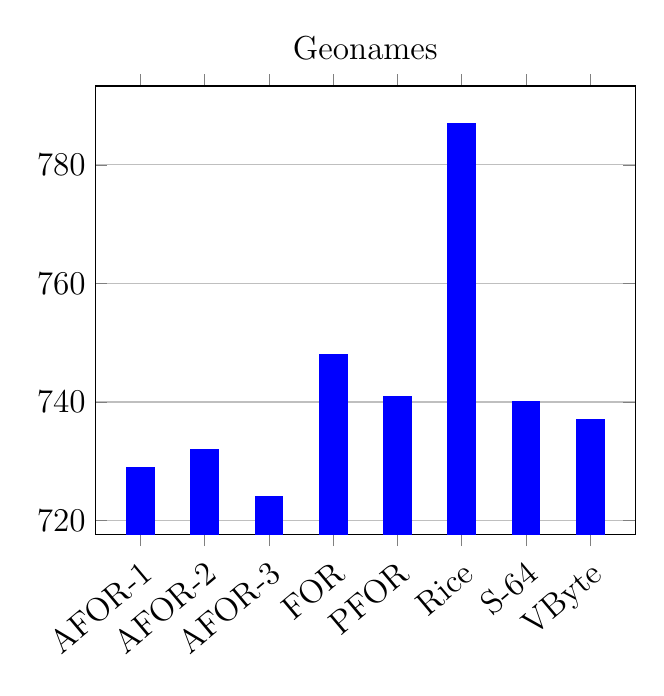
\begin{tikzpicture}[baseline]
\begin{axis}[
x tick label style={font=\large, rotate=40, anchor=north east},
xtick={1,...,8},
xticklabels={AFOR-1, AFOR-2, AFOR-3, FOR, PFOR, Rice, S-64, VByte},
legend style={at={(0.5,1.13)}, anchor=north, legend columns=-1},
label style={font=\large},
tick label style={font=\large},
title style={font=\large},
ybar,
ymajorgrids=true,
bar width=10pt,
title={Geonames},
%enlargelimits=0.15,
]
\addplot[draw=blue,fill=blue]
coordinates {(1, 729) (2, 732) (3, 724) (4, 748) (5, 741) (6, 787) (7, 740) (8, 737)};
%\legend{Blog}
\end{axis}
\end{tikzpicture}
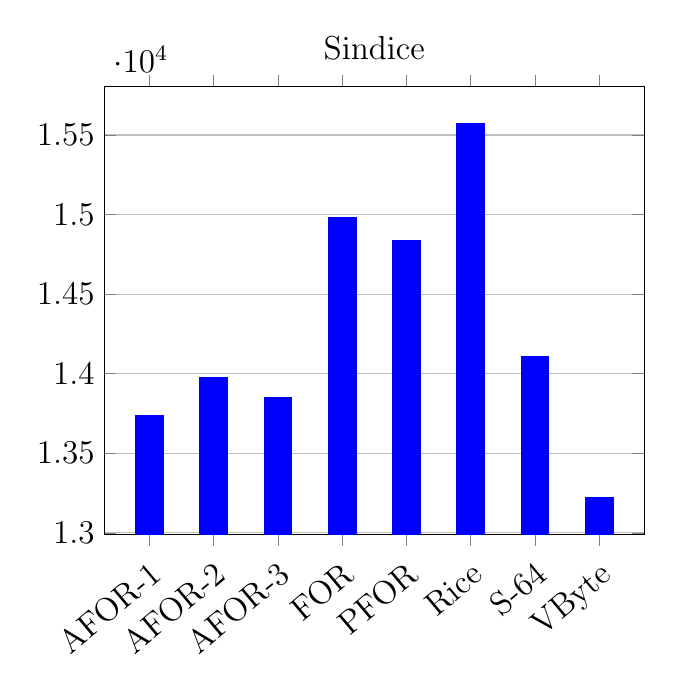
\begin{tikzpicture}[baseline]
\begin{axis}[
x tick label style={font=\large, rotate=40, anchor=north east},
xtick={1,...,8},
xticklabels={AFOR-1, AFOR-2, AFOR-3, FOR, PFOR, Rice, S-64, VByte},
legend style={at={(0.5,1.13)}, anchor=north, legend columns=-1},
label style={font=\large},
tick label style={font=\large},
title style={font=\large},
ybar,
ymajorgrids=true,
bar width=10pt,
title={Sindice},
%enlargelimits=0.15,
]
\addplot[draw=blue,fill=blue]
coordinates {(1, 13734) (2, 13975) (3, 13847) (4, 14978) (5, 14839) (6, 15571) (7, 14107) (8, 13223)};
%\legend{Blog}
\end{axis}
\end{tikzpicture}
% }
  }
	\caption{The total time spent to commit all the batches of 10000 document.}
	\label{fig:commit-time}
\end{figure}

\paragraph{Optimisation Time}

Figure~\ref{fig:optimise-time} shows the optimise time for each methods. The
time to perform the optimisation step is quite different due to the nature of
the operation. The optimisation operation has to read and decompress all the
index segments and compress them back into a single segment. Therefore,
decompression performance is also an important factor, and algorithms having
good decompression speed becomes more competitive.

On both data sources types, while PFOR was similar to Rice in term of commit
time on large datasets (Blog and Sindice), it is ahead of Rice in term of
optimisation time. This can be seen too with FOR on Sindice only. Rice is
penalised by its low decompression speed. The difference introduces by the
decompression performance can also be seen with S-6, which provides performance
close to or even better than VByte. While VByte performs fairly well on
unstructured data, we notice a large overhead on Sindice. The reason is the
distribution of the values on each stream: SIREn produce small values, since
there is a locality effect, i.e. attributes are local to an entity, values are
local to an attribute and positions are local to a value. On traditional
inverted index, position values are local to the whole document, and are then
much bigger. The Table~\ref{tab:indexing-performance} reports a positions
stream of size 20 GBytes at least with every compression techniques, while the
SIREn's streams sizes are bellow 2 GBytes. This difference in compression
ratio produce a large overhead on large datasets (Sindice) with the
decompression speed of VByte.

The best-performing methods are AFOR-1, AFOR-2 and AFOR-3 (structured data
only), with AFOR-3 performing better on large datasets. The AFOR techniques
take the advantage due their optimised compression and decompression routines
and their good compression rate. AFOR-3 is even twice as fast as Rice on the
Sindice dataset.

\begin{figure}
\centering
\begin{minipage}{0.8\linewidth}
  \centering
    \resizebox{0.7\linewidth}{!}{%
    % \subfloat[Unstructured data]{%
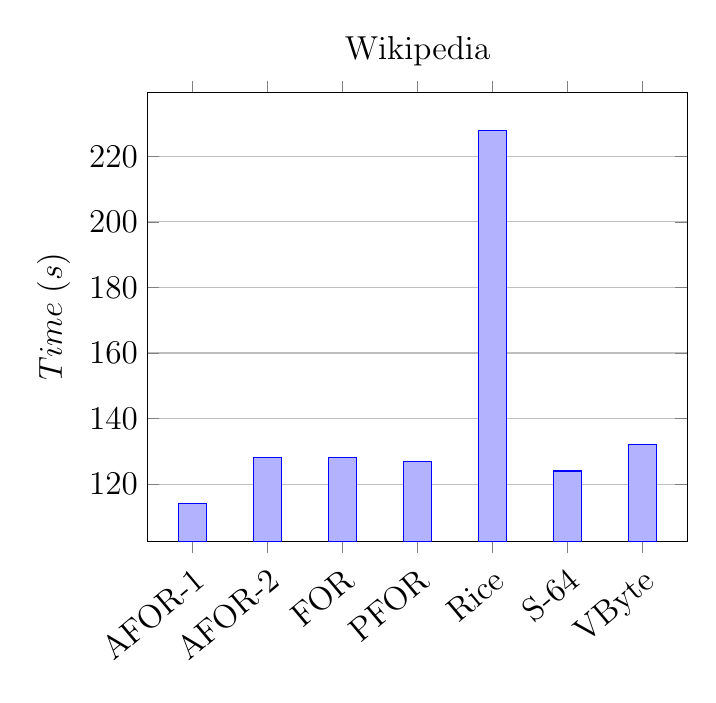
\begin{tikzpicture}[baseline]
\begin{axis}[
ylabel=$Time \; (s)$,
x tick label style={rotate=40, anchor=north east},
xtick={1,...,7},
xticklabels={AFOR-1, AFOR-2, FOR, PFOR, Rice, S-64, VByte},
legend style={at={(0.5,1.13)}, anchor=north, legend columns=-1},
label style={font=\large},
tick label style={font=\large},
title style={font=\large},
ybar,
ymajorgrids=true,
bar width=10pt,
title={Wikipedia},
%enlargelimits=0.15,
]
\addplot
coordinates {(1, 114) (2, 128) (3, 128) (4, 127) (5, 228) (6, 124) (7, 132)};
\end{axis}
\end{tikzpicture}%
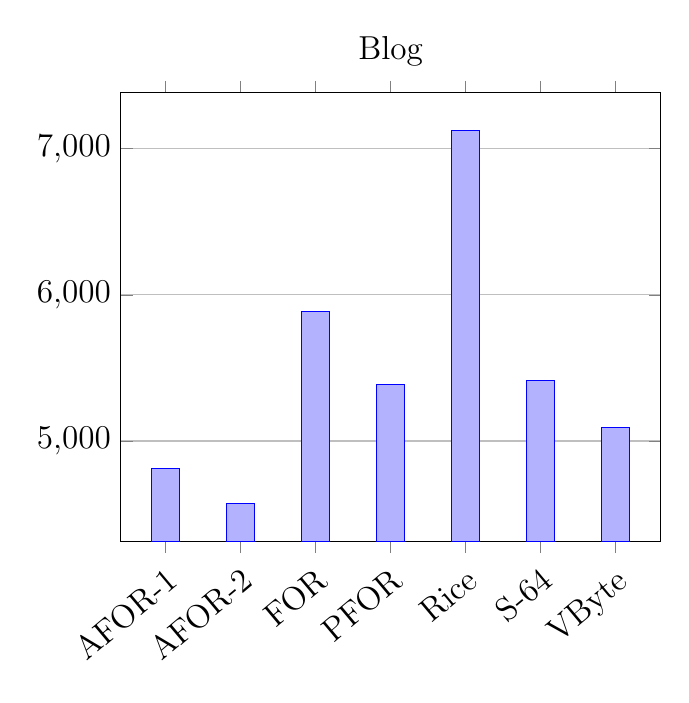
\begin{tikzpicture}[baseline]
\begin{axis}[
x tick label style={rotate=40, anchor=north east},
xtick={1,...,7},
xticklabels={AFOR-1, AFOR-2, FOR, PFOR, Rice, S-64, VByte},
legend style={at={(0.5,1.13)}, anchor=north, legend columns=-1},
label style={font=\large},
tick label style={font=\large},
title style={font=\large},
ybar,
ymajorgrids=true,
bar width=10pt,
title={Blog},
%enlargelimits=0.15,
]
\addplot
coordinates {(1, 4813) (2, 4571) (3, 5888) (4, 5387) (5, 7127) (6, 5414) (7,
5092)};
\end{axis}
\end{tikzpicture}
% }
  }
  \quad
  \resizebox{\linewidth}{!}{%
    % \subfloat[Structured data]{%
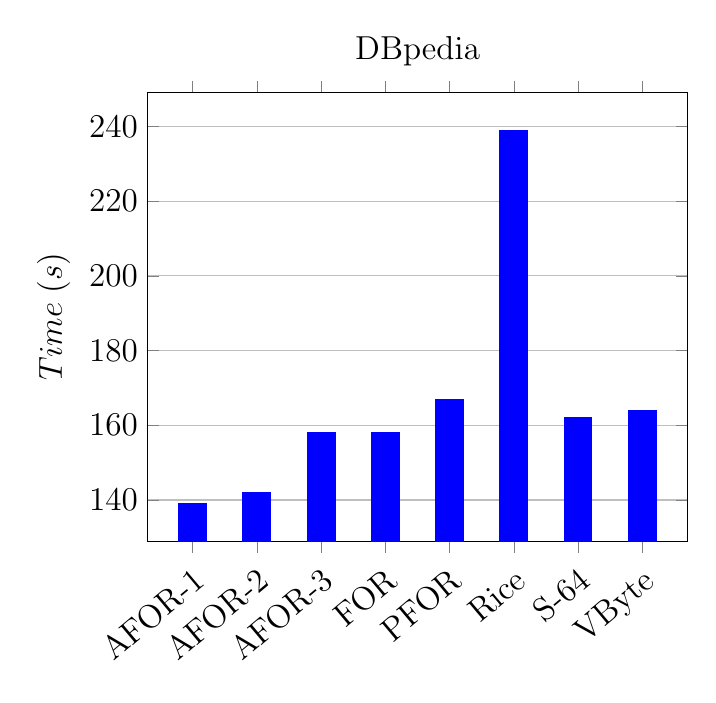
\begin{tikzpicture}[baseline]
\begin{axis}[
ylabel=$Time \; (s)$,
x tick label style={rotate=40, anchor=north east},
xtick={1,...,8},
xticklabels={AFOR-1, AFOR-2, AFOR-3, FOR, PFOR, Rice, S-64, VByte},
legend style={at={(0.5,1.13)}, anchor=north, legend columns=-1},
label style={font=\large},
tick label style={font=\large},
title style={font=\large},
ybar,
ymajorgrids=true,
bar width=10pt,
title={DBpedia},
%enlargelimits=0.15,
]
\addplot[draw=blue,fill=blue]
coordinates {(1, 139) (2, 142) (3, 158) (4, 158) (5, 167) (6, 239) (7, 162) (8, 164)};
\end{axis}
\end{tikzpicture}%
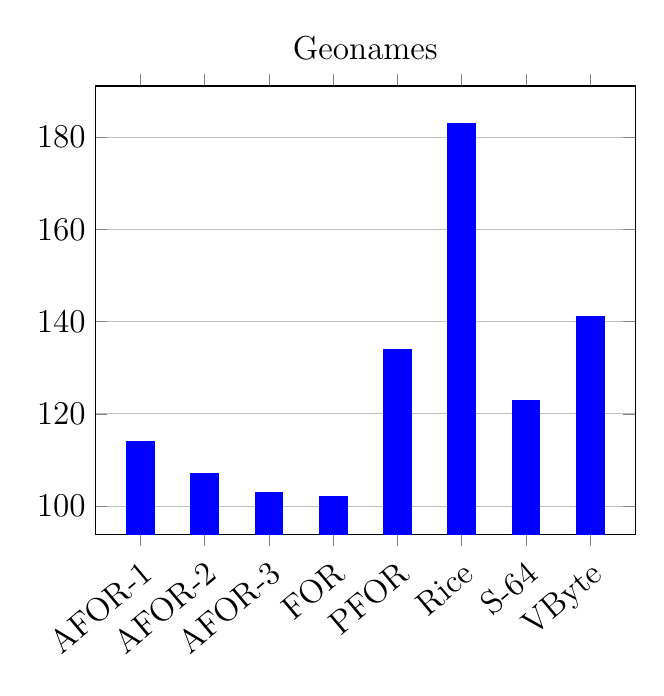
\begin{tikzpicture}[baseline]
\begin{axis}[
x tick label style={rotate=40, anchor=north east},
xtick={1,...,8},
xticklabels={AFOR-1, AFOR-2, AFOR-3, FOR, PFOR, Rice, S-64, VByte},
legend style={at={(0.5,1.13)}, anchor=north, legend columns=-1},
label style={font=\large},
tick label style={font=\large},
title style={font=\large},
ybar,
ymajorgrids=true,
bar width=10pt,
title={Geonames},
%enlargelimits=0.15,
]
\addplot[draw=blue,fill=blue]
coordinates {(1, 114) (2, 107) (3, 103) (4, 102) (5, 134) (6, 183) (7, 123) (8, 141)};
%\legend{Blog}
\end{axis}
\end{tikzpicture}
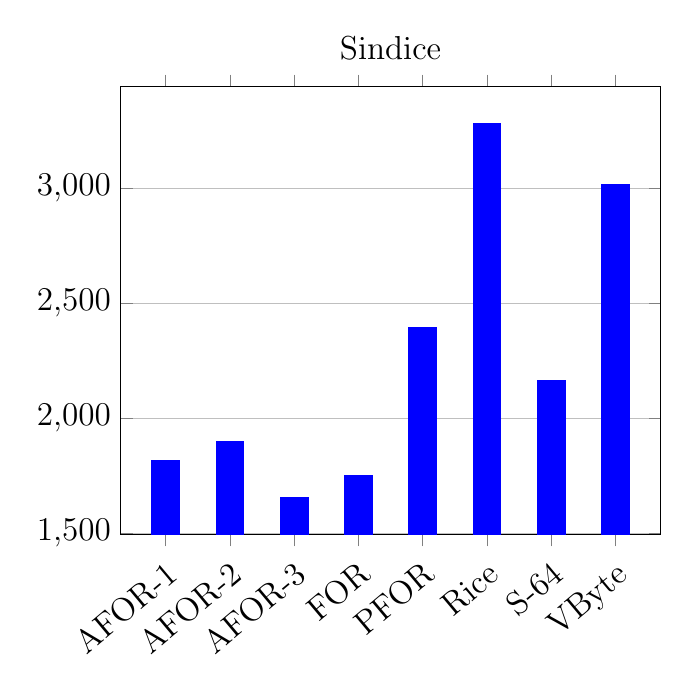
\begin{tikzpicture}[baseline]
\begin{axis}[
x tick label style={rotate=40, anchor=north east},
xtick={1,...,8},
xticklabels={AFOR-1, AFOR-2, AFOR-3, FOR, PFOR, Rice, S-64, VByte},
legend style={at={(0.5,1.13)}, anchor=north, legend columns=-1},
label style={font=\large},
tick label style={font=\large},
title style={font=\large},
ybar,
ymajorgrids=true,
bar width=10pt,
title={Sindice},
%enlargelimits=0.15,
]
\addplot[draw=blue,fill=blue]
coordinates {(1, 1816) (2, 1900) (3, 1656) (4, 1749) (5, 2396) (6, 3281) (7, 2163) (8, 3018)};
%\legend{Blog}
\end{axis}
\end{tikzpicture}
% }
  }
	\caption{The total time spent to optimise the complete index.}
	\label{fig:optimise-time}
\end{minipage}
\end{figure}

\paragraph{Compression Ratio}

Figure~\ref{fig:index-size} shows the total index size achieved by each
method. We can clearly see the inefficiency of the VByte approach. While VByte
performs generally better than FOR on traditional document-centric inverted
indexes like with Wikipedia and Blog datasets, this is not true for inverted
indexes based on a node indexing scheme like SIREn. VByte is not adapted to such
an index due to the properties of the delta-encoded lists of values. Apart
from the entity file, the values are generally very small and the outliers are
rare. In that case, VByte is penalized by its inability to encode a small
integer in less than a byte.

On the contrary, FOR is able to encode many small
integers in one byte. Also, while PFOR is less sensitive to outliers than FOR,
the gain of compression rate provided by PFOR is minimal since outliers are
more rare than in traditional inverted indexes. Indeed we can see that the
distribution of values with a document-centric indexing technique (Wikipedia
and Blog) lead to many outliers, and thus the PFOR algorithm is in that case
efficient.

In contrast, AFOR and S-64 are able to better adapt the encoding to
the value distribution and therefore provide a better compression rate. While
Rice provides the best compression ratio on traditional inverted indexes, AFOR
is able to provide better compression ratio than Rice on the Geonames and
Sindice dataset. Compared to AFOR-2, we can observe in
Table~\ref{tab:indexing-performance} that AFOR-3 provides better compression
rate on the frequency, value and position files, and slightly better on the
entity file. This result corroborates the existence of long runs of 1 in these
files, as explained in Section~\ref{sec:compression:stripping}.

In comparison to normal indexes, Rice provides worse compression ratio than
AFOR on a node indexing scheme index. This can be explained again by the small
values, since Rice does not compress long runs of small values as well as AFOR.

\begin{figure}
\centering
\begin{minipage}{0.8\linewidth}
  \centering
    \resizebox{0.7\linewidth}{!}{%
    % \subfloat[Unstructured data]{%
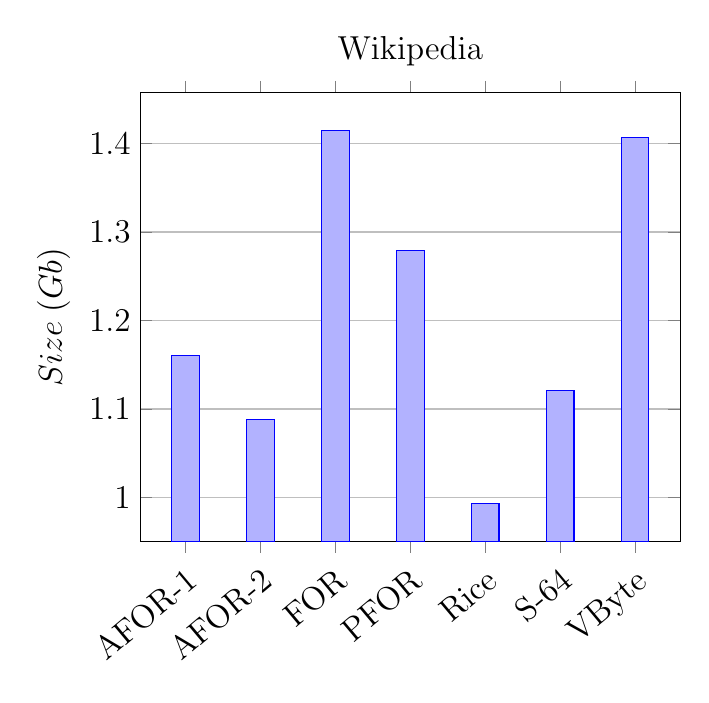
\begin{tikzpicture}[baseline]
\begin{axis}[
ylabel=$Size \; (Gb)$,
x tick label style={rotate=40, anchor=north east},
xtick={1,...,7},
xticklabels={AFOR-1, AFOR-2, FOR, PFOR, Rice, S-64, VByte},
legend style={at={(0.5,1.13)}, anchor=north, legend columns=-1},
label style={font=\large},
tick label style={font=\large},
title style={font=\large},
ybar,
ymajorgrids=true,
bar width=10pt,
title={Wikipedia},
%enlargelimits=0.15,
]
\addplot
coordinates {(1, 1.160) (2, 1.088) (3, 1.415) (4, 1.279) (5, 0.993) (6, 1.121)
(7, 1.407)};
\end{axis}
\end{tikzpicture}%

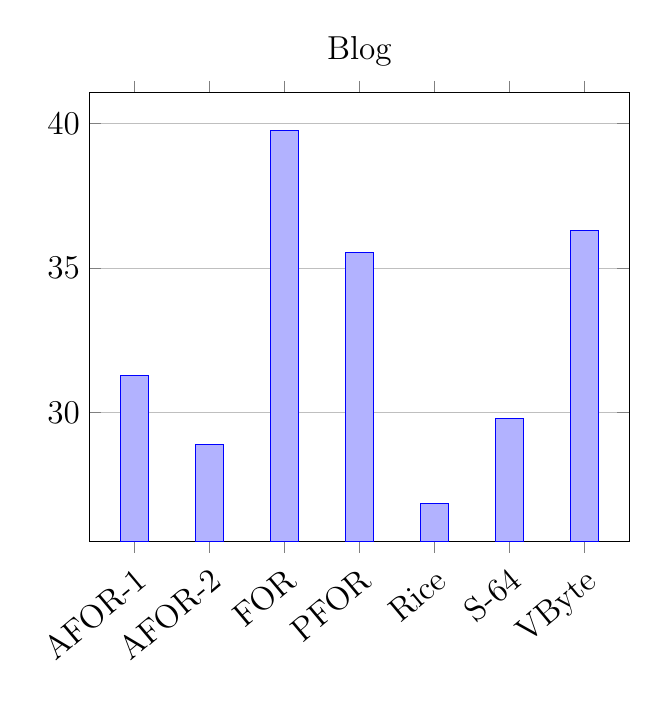
\begin{tikzpicture}[baseline]
\begin{axis}[
x tick label style={rotate=40, anchor=north east},
xtick={1,...,7},
xticklabels={AFOR-1, AFOR-2, FOR, PFOR, Rice, S-64, VByte},
legend style={at={(0.5,1.13)}, anchor=north, legend columns=-1},
label style={font=\large},
tick label style={font=\large},
title style={font=\large},
ybar,
ymajorgrids=true,
bar width=10pt,
title={Blog},
%enlargelimits=0.15,
]
\addplot
coordinates {(1, 31.292) (2, 28.895) (3, 39.777) (4, 35.536) (5, 26.851) (6,
29.800) (7, 36.303)};
\end{axis}
\end{tikzpicture}%
% }
  }
  \quad
  \resizebox{\linewidth}{!}{%
    % \subfloat[Unstructured data]{%
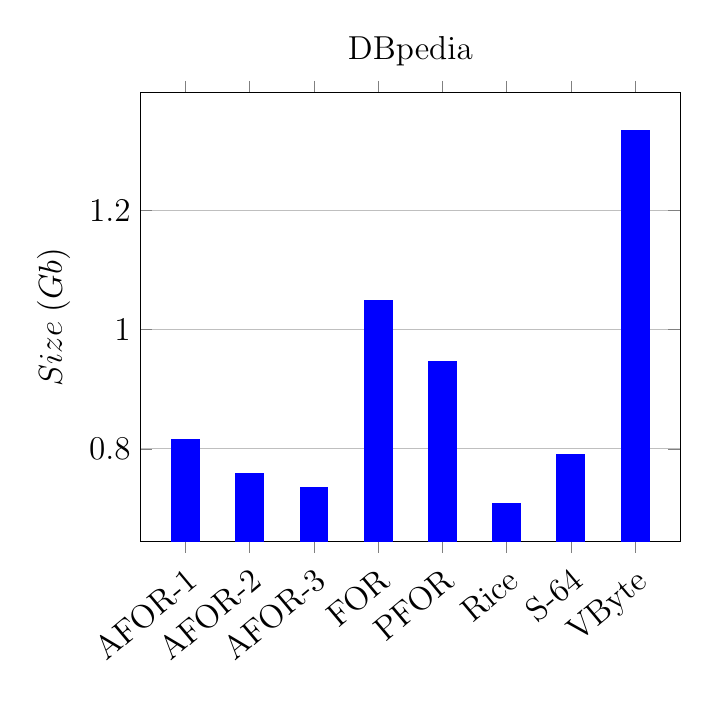
\begin{tikzpicture}[baseline]
\begin{axis}[
ylabel=$Size \; (Gb)$,
x tick label style={rotate=40, anchor=north east},
xtick={1,...,8},
xticklabels={AFOR-1, AFOR-2, AFOR-3, FOR, PFOR, Rice, S-64, VByte},
legend style={at={(0.5,1.13)}, anchor=north, legend columns=-1},
label style={font=\large},
tick label style={font=\large},
title style={font=\large},
ybar,
ymajorgrids=true,
bar width=10pt,
title={DBpedia},
%enlargelimits=0.15,
]
\addplot[draw=blue,fill=blue]
coordinates {(1, 0.816) (2, 0.758) (3, 0.736) (4, 1.049) (5, 0.946) (6, 0.708) (7, 0.791) (8, 1.335)};
\end{axis}
\end{tikzpicture}%
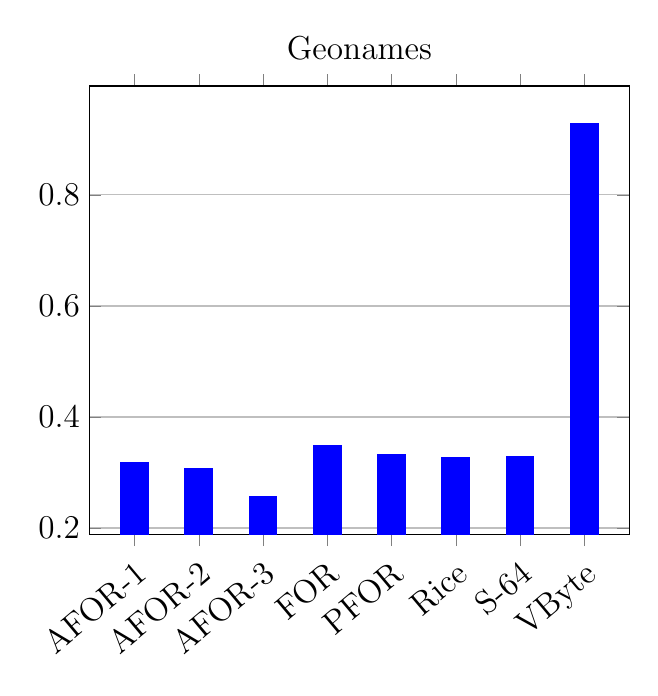
\begin{tikzpicture}[baseline]
\begin{axis}[
x tick label style={rotate=40, anchor=north east},
xtick={1,...,8},
xticklabels={AFOR-1, AFOR-2, AFOR-3, FOR, PFOR, Rice, S-64, VByte},
legend style={at={(0.5,1.13)}, anchor=north, legend columns=-1},
label style={font=\large},
tick label style={font=\large},
title style={font=\large},
ybar,
ymajorgrids=true,
bar width=10pt,
title={Geonames},
%enlargelimits=0.15,
]
\addplot[draw=blue,fill=blue]
coordinates {(1, 0.318) (2, 0.307) (3, 0.256) (4, 0.349) (5, 0.332) (6, 0.327) (7, 0.329) (8, 0.929)};
\end{axis}
\end{tikzpicture}%
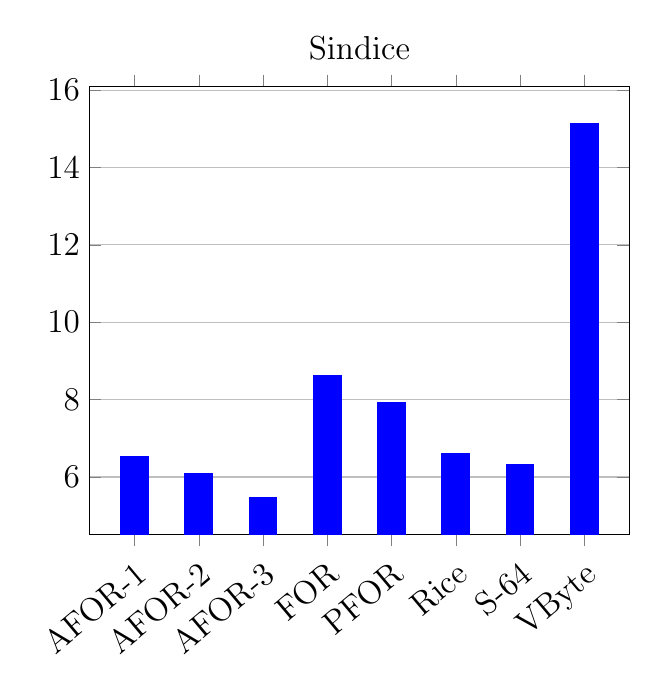
\begin{tikzpicture}[baseline]
\begin{axis}[
x tick label style={rotate=40, anchor=north east},
xtick={1,...,8},
xticklabels={AFOR-1, AFOR-2, AFOR-3, FOR, PFOR, Rice, S-64, VByte},
legend style={at={(0.5,1.13)}, anchor=north, legend columns=-1},
label style={font=\large},
tick label style={font=\large},
title style={font=\large},
ybar,
ymajorgrids=true,
bar width=10pt,
title={Sindice},
%enlargelimits=0.15,
]
\addplot[draw=blue,fill=blue]
coordinates {(1, 6.537) (2, 6.082) (3, 5.475) (4, 8.611) (5, 7.924) (6, 6.605) (7, 6.313) (8, 15.132)};
\end{axis}
\end{tikzpicture}%
% }
  }
	\caption{The index size achieved by each compression technique.}
	\label{fig:index-size}
\end{minipage}
\end{figure}

\paragraph{Conclusion on Indexing Performance}

The indexing experiment shows that the compression speed is also an important
factor to take into consideration when designing a compression algorithm for
an inverted index. Without a good compression speed, the update throughput of
the index is limited. Also the experiment shows that the optimisation
operation is dependent of the decompression performance, and its execution
time can double without a good compression and decompression speed. With
respect to index optimisation, the compression ratio must also be taken into
consideration. While VByte provides in general correct commit times, we can
observe on a large dataset (Sindice) that its performance during optimisation
is limited by its poor compression ratio.

Overall, the method providing the best balance between indexing time, optimise
time and compression ratio is the AFOR family, and this on both structured and
unstructured datasets. AFOR-1 provides fast compression speed and better
compression ratio than FOR and PFOR. AFOR-2 provides a notable additional gain
in compression ratio and optimise time but undergoes a slight increase of
indexing time. AFOR-3 provides another additional gain in compression ratio
while providing better compression speed than AFOR-2.

\section{Querying Performance}
\label{sec:compression:query-performance}

We now compare the decompression performance in real settings, where inverted
indexes are answering queries of various complexities. We report in this
section only the benchmarks done on structured datasets (DBpedia,
Geonames and Sindice), since the performance of query processing on unstructured
datasets is comparable to the ones run on the structured datasets and for
question of clarity also. The raw results are nonetheless reported in the
appendix in the Table~\ref{tab:query-time-TRAD}.

We focus on two main classes of queries, the value and attribute queries, which
are the core elements of a star-shaped query. Among these two classes, we
identify types of keyword queries which represent the common queries received
by a web search engine: conjunction, disjunction and phrase.

\subsection{Query Benchmarking Framework}
\label{sec:bench-query-FW}

In this section we present the types of queries that are run against indexes
compressed with different algorithms.

\subsection{Query Generation}

The queries are generated based on the selectivity of the words composing
them. The word selectivity determines how many entities match a given keyword.
The words are grouped into three selectivity ranges: \emph{high}, \emph{medium}
and \emph{low}. We differentiate also two groups of
words based on their position in the data graph: attribute and value. We
follow the technique described in \cite{errcegovac:2005:vldb} to obtain the
ranges of each word group. We first order the words by their descending
frequency, and then take the first $k$ words whose cumulative frequency is
90\% of all word occurrences as high range. The medium range accounts for the
next 10\%, and the low range is composed of all the remaining words. For the
phrase queries, we follow a similar technique. We first extract all the 2-gram
and 3-gram\footnote{A n-gram is $n$ words that appear contiguously} from the
data collection. We then compute their frequency and sort them by descending
frequency. We finally create the three ranges as explained above. Benchmarks
involving queries with words from low and medium ranges are not reported here
for questions of space, but the performance results are comparable with the
one presented here.

\subsubsection{Value Queries}

Value queries are divided into three types of keyword queries:
\emph{conjunction}, \emph{disjunction} and \emph{phrase} queries. These queries
are restricted to match within one single value, e.g. to find all entities
which have the word ``fantasy'' within a value as in \ref{fig:entities}.
Therefore, the processing of conjunction and disjunction queries relies on the
entity, frequency, attribute and value inverted files. Phrase queries rely on
one additional stream, the position values.

Conjunction and disjunction queries are generated by taking random keywords
from the high range group of words. 2-AND and 2-OR (resp. 4-AND and 4-OR)
denotes conjunction and disjunction queries with 2 random keywords (resp. 4
random keywords). Similarly, a phrase query is generated by taking random
n-grams from the high range group. 2-Phrase (resp. 3-Phrase) denotes phrase
queries with 2-gram (resp. 3-gram). Benchmarks involving queries with words
from low and medium ranges are not reported here for questions of space, but
the performance results are comparable with the ones presented here.

\subsubsection{Attribute Queries}

An attribute query is generated by associating one attribute keyword with one
value query. An attribute keyword is randomly chosen from the high range
groups of attribute words. The associated value query is obtained as explained
previously. An attribute query intersects the result of a value query with an
attribute keyword.

\subsection{Query Benchmark Design}

The benchmarking design used is the one presented in the
Chapter~\ref{chap:benchmarking-framework}. For each type of query, we 
\begin{inparaenum}[(1)]
\item generate a set of 200 random queries which is reused for all the
compression methods, and
\item perform 100 measurements.
\end{inparaenum}
All measurements are made using \emph{warm cache}, i.e., the part of the index
read during query processing is fully loaded in memory.

Query execution time is sensitive to external events which can affect the
final execution time recorded.
% For instance, background system maintenance or
% interruptions as well as cache misses or system exceptions can occur and
% perturb the measurements. All these events are unpredictable and must be
% treated as noise. Therefore, we need to quantify the accuracy of our
% measurements.
% As recommended in \cite{lilja:2000:book}, we report the
% arithmetic mean and the standard deviation of the 100 measurements.
To assess differences between the algorithms, confidence intervals with 95\%
degree of confidence have been used.  The design of the value and attribute
query benchmarks includes three factors:
\begin{description}
\item[Algorithm] having height levels: AFOR-1, AFOR-2, AFOR-3, FOR, PFOR,
Rice, S-64, and VByte;
\item[Query] having six levels: 2-AND, 2-OR, 4-AND, 4-OR, 2-Phrase, and
3-Phrase; and
\item[Dataset] having three levels: DBpedia, Geonames and Sindice. 
\end{description}
Each condition of the design, e.g., AFOR-1 / 2-AND / DBpedia, contains 100
separate measurements.

\subsection{Query Benchmark Results}

We report the results of the query benchmarks in
Table~\ref{tab:value-query-time} and Table~\ref{tab:attribute-query-time} in
the appendix for the value and attribute queries respectively. Based on these
results, we derive multiple graphical charts to better visualise the
differences between each algorithm. These charts are then used to compare and
discuss the performances of each algorithm.

Figure~\ref{fig:avg-value-query-time} and
Figure~\ref{fig:avg-attribute-query-time} report the average query processing
time for the value and attribute queries respectively.
Figure~\ref{fig:avg-value-boolean-query-time} and
Figure~\ref{fig:avg-attribute-boolean-query-time} depict the average
processing time on the Boolean queries.
Figure~\ref{fig:avg-value-phrase-query-time} and
Figure~\ref{fig:avg-attribute-phrase-query-time} depict the average processing
time on the phrase queries (2-Phrase, 3-Phrase). The query processing time are
obtained by summing up the average time of each query from
Table~\ref{tab:value-query-time} for the value queries and
Table~\ref{tab:attribute-query-time} for the attribute queries. For example,
the processing time of AFOR-1 on the DBpedia dataset in
Figure~\ref{fig:avg-value-phrase-query-time} is obtained by summing up the
processing times of the queries 2-Phrase (43.2 ms) and 3-Phrase (32.6 ms)
reported in Table~\ref{tab:value-query-time} in the appendix.

\paragraph{Value Query}

In Figure~\ref{fig:avg-value-query-time}, and in particular on the Sindice
dataset (large dataset), we can distinguish three classes of algorithms: the
techniques based on FOR, a group composed of S-64 and VByte, and finally Rice.
The FOR group achieves relatively similar results, with AFOR-2 slightly behind
the others.

Rice has the worst performance for every query and dataset, followed by VByte.
Nonetheless Rice performs in many cases twice as slow as VByte. In
Figure~\ref{fig:avg-value-boolean-query-time}, S-64 provides similar
performance to VByte on Boolean queries but we can see in
Figure~\ref{fig:avg-value-phrase-query-time} that it is faster than VByte on
phrase queries. However, S-64 stays behind FOR, PFOR and AFOR in all the cases.

FOR, PFOR and AFOR have relatively similar performances on all the Boolean
queries and all the datasets. PFOR seems to provide generally slightly better
performance on the phrase queries but seems to be slower on Boolean queries.

\begin{figure}
  \centering
  \subfloat[Boolean Query]{%
    \resizebox{0.45\linewidth}{!}{%
      
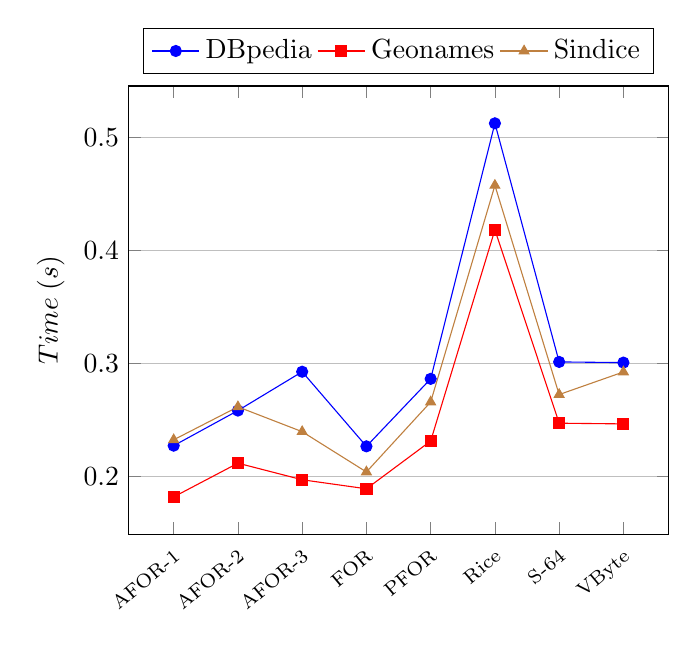
\begin{tikzpicture}
\begin{axis}[
ylabel=$Time \; (s)$,
x tick label style={font=\scriptsize, rotate=40, anchor=north east},
xtick={1,...,8},
xticklabels={AFOR-1, AFOR-2, AFOR-3, FOR, PFOR, Rice, S-64, VByte},
legend style={at={(0.5,1.13)}, anchor=north, legend columns=-1},
%ybar,
ymajorgrids=true,
%bar width=5pt,
]

\addplot[blue,mark=*]
coordinates {(1, 0.2271) (2, 0.2582) (3, 0.2926) (4, 0.2265) (5, 0.2863) (6, 0.5127) (7, 0.3013) (8, 0.3007)};
\addplot[red,mark=square*]
coordinates {(1, 0.1817) (2, 0.2116) (3, 0.1969) (4, 0.1889) (5, 0.2312) (6, 0.4184) (7, 0.2470) (8, 0.2464)};
\addplot[brown,mark=triangle*]
coordinates {(1, 0.2323) (2, 0.2615) (3, 0.2395) (4, 0.2038) (5, 0.2658) (6, 0.4577) (7, 0.2724) (8, 0.2924)};

\legend{DBpedia, Geonames, Sindice}

\end{axis}
\end{tikzpicture}%

  	}
  	\label{fig:avg-value-boolean-query-time}
  }\quad%
  \subfloat[Phrase Query]{%
    \resizebox{0.45\linewidth}{!}{%
      
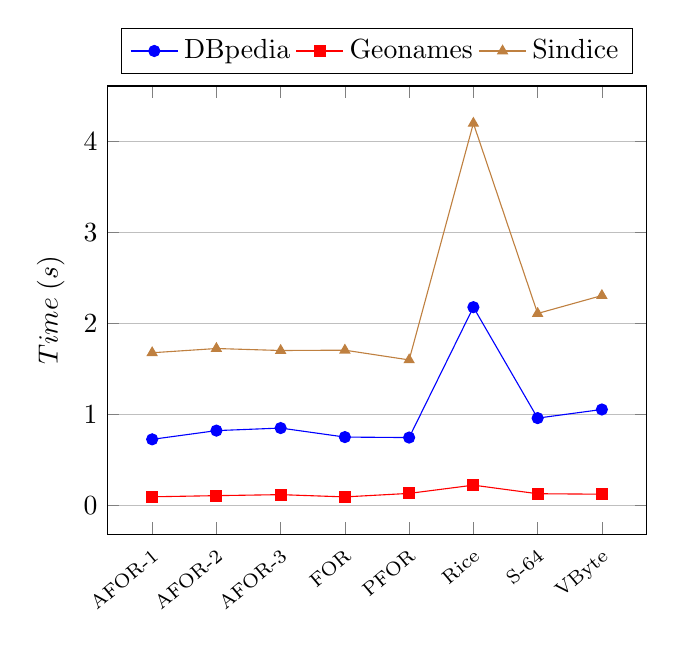
\begin{tikzpicture}
\begin{axis}[
ylabel=$Time \; (s)$,
x tick label style={font=\scriptsize, rotate=40, anchor=north east},
xtick={1,...,8},
xticklabels={AFOR-1, AFOR-2, AFOR-3, FOR, PFOR, Rice, S-64, VByte},
legend style={at={(0.5,1.13)}, anchor=north, legend columns=-1},
%ybar,
ymajorgrids=true,
%bar width=5pt,
]

\addplot[blue,mark=*]
coordinates {(1, 0.7267) (2, 0.8225) (3, 0.8506) (4, 0.7516) (5, 0.7462) (6, 2.1778) (7, 0.9598) (8, 1.0544) };
\addplot[red,mark=square*]
coordinates {(1, 0.0959) (2, 0.1085) (3, 0.1196) (4, 0.0947) (5, 0.1333) (6, 0.2237) (7, 0.1296) (8, 0.1245)};
\addplot[brown,mark=triangle*]
coordinates {(1, 1.6773) (2, 1.7239) (3, 1.702) (4, 1.7056) (5, 1.5986) (6, 4.1963) (7, 2.1086) (8, 2.3053)};

\legend{DBpedia, Geonames, Sindice}

\end{axis}
\end{tikzpicture}%

    }
    \label{fig:avg-value-phrase-query-time}
  }%
	\caption{The average processing time for the value queries that is achieved
	by each compression technique.}
	\label{fig:avg-value-query-time}
\end{figure}

\paragraph{Attribute Query}

In Figure~\ref{fig:avg-attribute-query-time}, and in particular on Sindice, we
can again distinguish the same three classes of algorithms. However, the
performance gap between S-64 and VByte becomes wider.

Rice has again the worst performance for every query and dataset. Compared to
the performance on value queries, we can see in
Figure~\ref{fig:avg-attribute-boolean-query-time} that S-64 provides similar
performance to PFOR and AFOR-2 on Boolean queries. FOR and AFOR-3 seem to be
the best performing methods on Boolean queries. With respect to the phrase
queries in Figure~\ref{fig:avg-attribute-phrase-query-time}, S-64 has better
performance than VByte. However, PFOR does not achieve any more the best
performance on phrase queries. Instead, it seems that AFOR-2 and FOR achieve a
slightly better processing time.

FOR, PFOR and AFOR have again relatively similar performances on all the
queries and all the datasets. AFOR-2 appears to be slower to some degree,
while the gap between AFOR-3 and PFOR becomes less perceptible.

\begin{figure}
  \centering
  \subfloat[Boolean Query]{%
    \resizebox{0.45\linewidth}{!}{%
      
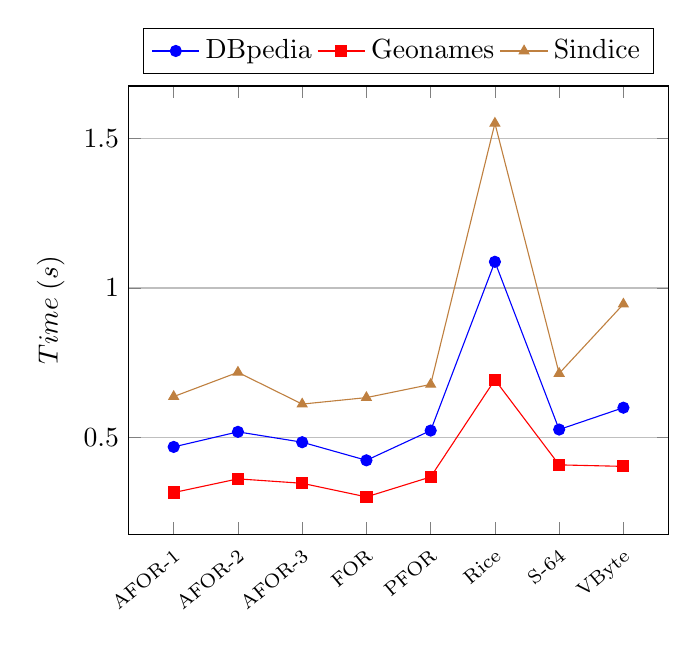
\begin{tikzpicture}
\begin{axis}[
ylabel=$Time \; (s)$,
x tick label style={font=\scriptsize, rotate=40, anchor=north east},
xtick={1,...,8},
xticklabels={AFOR-1, AFOR-2, AFOR-3, FOR, PFOR, Rice, S-64, VByte},
legend style={at={(0.5,1.13)}, anchor=north, legend columns=-1},
%ybar,
ymajorgrids=true,
%bar width=7pt,
]

\addplot[blue,mark=*]
coordinates {(1, 0.4692) (2, 0.5195) (3, 0.4849) (4, 0.4244) (5, 0.5238) (6, 1.0875) (7, 0.5272) (8, 0.6002)};
\addplot[red,mark=square*]
coordinates {(1, 0.3167) (2, 0.3625) (3, 0.3477) (4, 0.3022) (5, 0.3689) (6, 0.6936) (7, 0.4092) (8, 0.4042)};
\addplot[brown,mark=triangle*]
coordinates {(1, 0.6373) (2, 0.7183) (3, 0.6122) (4, 0.6339) (5, 0.6779) (6, 1.55) (7, 0.7146) (8, 0.946)};

\legend{DBpedia, Geonames, Sindice}

\end{axis}
\end{tikzpicture}


  	}
  	\label{fig:avg-attribute-boolean-query-time}
  }\quad%
  \subfloat[Phrase Query]{%
    \resizebox{0.45\linewidth}{!}{%
      
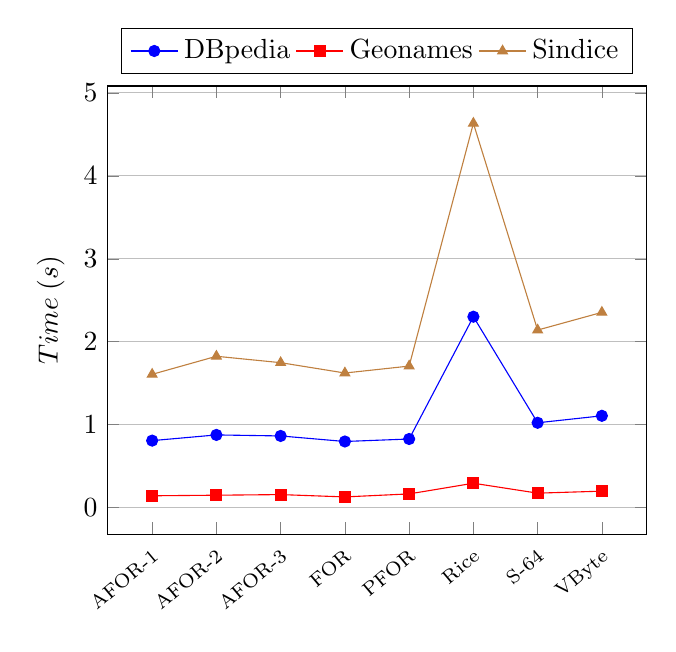
\begin{tikzpicture}
\begin{axis}[
ylabel=$Time \; (s)$,
x tick label style={font=\scriptsize, rotate=40, anchor=north east},
xtick={1,...,8},
xticklabels={AFOR-1, AFOR-2, AFOR-3, FOR, PFOR, Rice, S-64, VByte},
legend style={at={(0.5,1.13)}, anchor=north, legend columns=-1},
%ybar,
ymajorgrids=true,
%bar width=7pt,
]

\addplot[blue,mark=*]
coordinates {(1, 0.8081) (2, 0.8767) (3, 0.8644) (4, 0.7976) (5, 0.8275) (6, 2.302) (7, 1.0232) (8, 1.1072)};
\addplot[red,mark=square*]
coordinates {(1, 0.143) (2, 0.1499) (3, 0.1574) (4, 0.1293) (5, 0.1656) (6, 0.2943) (7, 0.1747) (8, 0.1988)};
\addplot[brown,mark=triangle*]
coordinates {(1, 1.6073) (2, 1.825) (3, 1.7478) (4, 1.6231) (5, 1.7067) (6, 4.6336) (7, 2.1409) (8, 2.3544)};

\legend{DBpedia, Geonames, Sindice}

\end{axis}
\end{tikzpicture}


    }
    \label{fig:avg-attribute-phrase-query-time}
  }%
	\caption{The average processing time for the attribute queries that is
	achieved by each compression technique.}
	\label{fig:avg-attribute-query-time}
\end{figure}

\section{Performance Trade-Off}

We report in Figure~\ref{fig:trade-off-time-bytes} the trade-off between the
total query processing time and the compression ratio among all the techniques
on the Sindice dataset. The total query time has been obtained by summing up
the average time of all the queries. The compression ratio is based on the
number of bytes read during query processing which are reported in
Table~\ref{tab:value-query-time} and Table~\ref{tab:attribute-query-time} in
the appendix.
We can distinctively see that the AFOR techniques are close to Rice in term of
compression ratio, while being relatively close to FOR and PFOR in term of
query processing time. Compared to AFOR-1, AFOR-2 achieves a better
compression rate in exchange of a slightly slower processing time. However,
AFOR-3 accomplishes a better compression rate with a processing time close to
AFOR-1.

\begin{figure}
  \centering
  \subfloat[Value Query]{%
    \resizebox{0.47\linewidth}{!}{%
      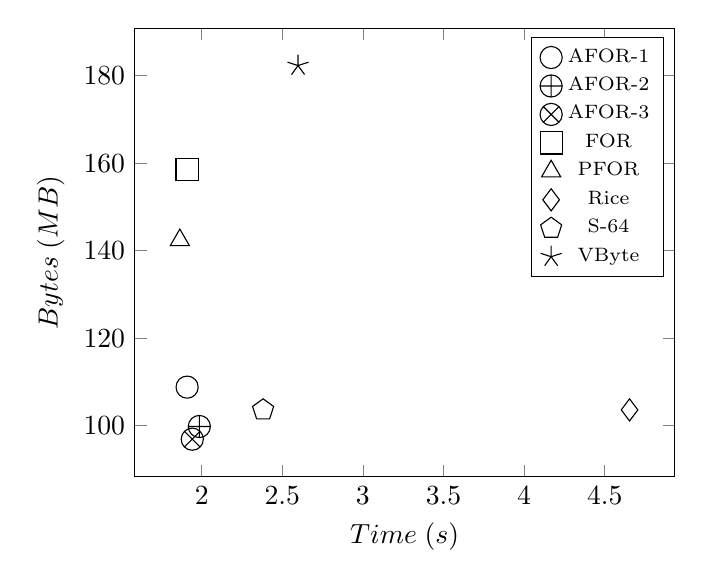
\begin{tikzpicture}
\begin{axis}[
scatter/classes={
	a={mark=o},
	b={mark=oplus},
	c={mark=otimes},
	d={mark=square},
	e={mark=triangle},
	f={mark=diamond},
	g={mark=pentagon},
	h={mark=star}
  },
  ylabel=$Bytes \; (MB)$,
  xlabel=$Time \; (s)$,
  mark options={scale=2},
  legend style={font=\scriptsize}
]

\addplot[scatter, only marks]
plot[scatter src=explicit symbolic]
coordinates {
(1.9096, 108.8) [a]
(1.9854, 99.8) [b]
(1.9415, 96.9) [c]
(1.9094, 158.5) [d]
(1.8644, 142.4) [e]
(4.654, 103.6) [f]
(2.381, 103.6) [g]
(2.5977, 182.3) [h]
};

\legend{AFOR-1, AFOR-2, AFOR-3, FOR, PFOR, Rice, S-64, VByte}

\end{axis}
\end{tikzpicture}
  	}
  }%
  \subfloat[Attribute Query]{%
    \resizebox{0.47\linewidth}{!}{%
      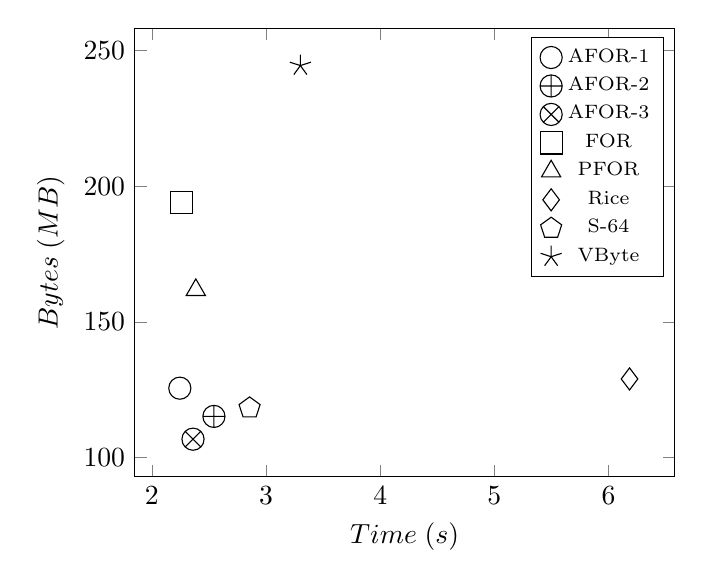
\begin{tikzpicture}
\begin{axis}[
	scatter/classes={
	a={mark=o},
	b={mark=oplus},
	c={mark=otimes},
	d={mark=square},
	e={mark=triangle},
	f={mark=diamond},
	g={mark=pentagon},
	h={mark=star}
  },
  ylabel=$Bytes \; (MB)$,
  xlabel=$Time \; (s)$,
  mark options={scale=2},
  legend style={font=\scriptsize},
]

\addplot[only marks]
plot[scatter, scatter src=explicit symbolic]
coordinates {
 (2.2446, 125.6) [a]
 (2.5433, 115.2) [b]
 (2.36, 106.8) [c]
 (2.257, 194.0) [d]
 (2.3846, 161.8) [e]
 (6.1836, 129.0) [f]
 (2.8555, 118.3) [g]
 (3.3004, 244.5) [h]
};
\legend{AFOR-1, AFOR-2, AFOR-3, FOR, PFOR, Rice, S-64, VByte}
\end{axis}
\end{tikzpicture}
    }
  }%
	\caption{A graphical comparison showing the trade-off between querying time
	and compression ratio on the Sindice dataset. The compression ratio is
	represented by the number of bytes read during the query processing.}
	\label{fig:trade-off-time-bytes}
\end{figure}

We report in Figure~\ref{fig:trade-off-query-update} the trade-off between the
total query processing time and the indexing time among all the techniques on
the Sindice dataset. The indexing time has been obtained by summing up the
commit and optimise time from Table~\ref{tab:indexing-performance} of the
appendix. We can distinctively see that the AFOR techniques achieve the best
trade-off between indexing and querying time. AFOR-3 produce very similar
indexing and querying times to AFOR-1, while providing a much better
compression rate. It is interesting to notice that PFOR provides a slightly
better querying time than FOR but at the price of a much slower compression.
Also, S-64 and VByte provide a relatively close performance trade-off. To
conclude, AFOR-3 seems to offer the best compromise between querying time,
indexing time, and compression rate.

\begin{figure}
  \centering
  \subfloat[Value Query]{%
    \resizebox{0.47\linewidth}{!}{%
      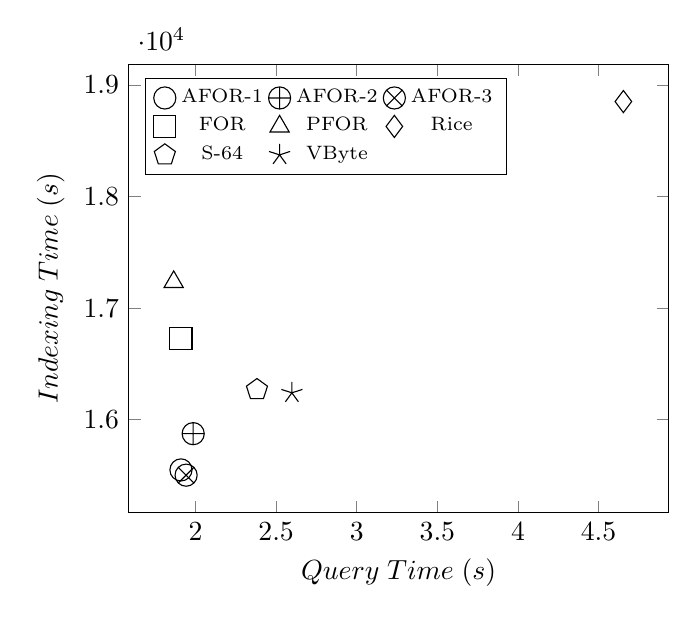
\begin{tikzpicture}
\begin{axis}[%
  scatter/classes={%
	a={mark=o},%
	b={mark=oplus},%
	c={mark=otimes},%
	d={mark=square},%
	e={mark=triangle},%
	f={mark=diamond},%
	g={mark=pentagon},%
	h={mark=star}
  },
  ylabel=$Indexing \; Time \; (s)$,
  xlabel=$Query \; Time \; (s)$,
  mark options={scale=2},
  legend columns=3,
  legend pos=north west,
  legend style={font=\scriptsize, anchor=north west, legend columns=3},
]

\addplot[only marks]
plot[scatter,scatter src=explicit symbolic]
coordinates {%
(1.9096, 15550) [a]
(1.9854, 15875) [b]
(1.9415, 15503) [c]
(1.9094, 16727) [d]
(1.8644, 17235) [e]
(4.654, 18852) [f]
(2.381, 16270) [g]
(2.5977, 16241) [h]
};%
\legend{AFOR-1, AFOR-2, AFOR-3, FOR, PFOR, Rice, S-64, VByte}
\end{axis}
\end{tikzpicture}
  	}
  }%
  \subfloat[Attribute Query]{%
    \resizebox{0.47\linewidth}{!}{%
      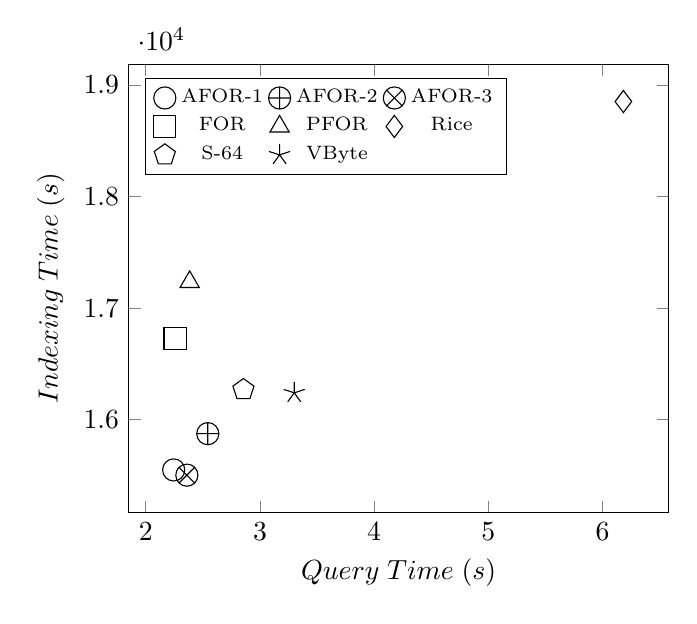
\begin{tikzpicture}
\begin{axis}[
  scatter/classes={
	a={mark=o},%
	b={mark=oplus},%
	c={mark=otimes},%
	d={mark=square},%
	e={mark=triangle},%
	f={mark=diamond},%
	g={mark=pentagon},%
	h={mark=star}
  },
  ylabel=$Indexing \; Time \; (s)$,
  xlabel=$Query \; Time \; (s)$,
  mark options={scale=2},
  legend columns=3,
  legend pos=north west,
  legend style={font=\scriptsize, anchor=north west, legend columns=3}
]

\addplot[only marks]
plot[scatter,mark=*,scatter src=explicit symbolic]
coordinates {
(2.2446, 15550) [a]
(2.5433, 15875) [b]
(2.3600, 15503) [c]
(2.2570, 16727) [d]
(2.3846, 17235) [e]
(6.1836, 18852) [f]
(2.8555, 16270) [g]
(3.3004, 16241) [h]
};
\legend{AFOR-1, AFOR-2, AFOR-3, FOR, PFOR, Rice, S-64, VByte}
\end{axis}
\end{tikzpicture}
    }
  }%
\caption{A graphical comparison of the compression techniques showing the
trade-off between querying time and indexing time on the Sindice dataset.}
\label{fig:trade-off-query-update}
\end{figure}

\section{Discussion}

In general, even if FOR has more data to read and decompress, it still
provides one of the best query execution time. The reason is that our
experiments are performed using warm cache. We therefore ignore the cost of
disk IO accesses and measure exclusively the decompression efficiency of the
methods. With a cold cache, i.e., when IO disk accesses have to be performed,
we expect a drop of performance for algorithms with a low compression ratio
such as FOR and PFOR compared to AFOR-2 and AFOR-3.

Compression and decompression performance do not only depend on the
compression ratio, but also on the execution flow of the algorithm and on the
number of cycles needed to compress or decompress an integer. Therefore,
CPU-optimised algorithms which provides at the same time a good compression
ratio are most likely to increase the update and query throughput of web
search engines. In that context, AFOR seems to be a good candidate since it is
well balanced in all aspects: it provides very good indexing and querying
performance and one of the best compression ratio.

The Simple encoding family is somehow similar to AFOR. At each iteration, S-64
encodes or decodes a variable number of integers using CPU optimised routines.
AFOR is however not tied to the size of a machine word, and is thus simpler to
implement and provides better compression ratio, compression speed and
decompression speed.
